\chapter{Clustering---The Emergence of Natural Kinds}

\begin{quote}
    \itshape
    ``The whole is other than the sum of its parts.''
    
    % (removed leading Markdown code fence)
\end{quote}

\begin{quote}
    \itshape
    ``Analysis is the mental process by which we ascend from effects to causes.''
    
    \raggedleft--- Classical Epistemology
\end{quote}

\section{Introduction: Data as Seeds of Knowledge}

\subsection{The Philosophical Foundation of Clustering}

In the landscape of machine learning, clustering occupies a unique philosophical position. Unlike supervised learning, which imposes external categories upon data, clustering allows \textit{structure to emerge from within}---revealing what Plato would call the ``natural kinds'' hidden in the phenomena.

\begin{philobox}
\textbf{Data as Initial Elements of Knowledge}

Every datum is a \textit{seed of knowledge}---a potential that requires proper nurturing and contextualization to reveal its essence. Just as Aristotle distinguished between potentiality (\textit{dynamis}) and actuality (\textit{energeia}), raw data exist in a state of epistemic potentiality, awaiting the analytical process to actualize their meaning.

Clustering is the method by which we move from the \textit{many} (individual data points) to the \textit{few} (cluster prototypes), and ultimately to the \textit{one} (underlying structure). This mirrors the Neoplatonic process of \textit{epistrophe}---the return from multiplicity to unity.
\end{philobox}

\subsection{From Effects to Causes: The Epistemology of Analysis}

Classical epistemology teaches that analysis is the intellectual ascent from observable effects to their hidden causes. When we observe that certain customers purchase similar products, certain genes co-express in disease states, or certain galaxies cluster in cosmic voids, we are witnessing \textit{effects}---the downstream consequences of underlying causal mechanisms.

Clustering formalizes this ascent through mathematical rigor:

\begin{equation}
    \text{Observable Data} \xrightarrow{\text{Clustering}} \text{Latent Structure} \xrightarrow{\text{Interpretation}} \text{Causal Hypotheses}
\end{equation}

\begin{remark}[Determinism and Epistemic Limits]
If we possessed perfect information about all causal factors (Laplace's demon), clustering would reveal the ``true'' structure with no ambiguity. However, practical limitations---measurement noise, missing features, finite sample sizes---introduce \textit{irreducible error}. This is not a failure of the algorithm but a fundamental constraint of epistemic finitude.
\end{remark}

\section{K-Means Clustering: Optimization as Discovery}

\subsection{The Mathematical Formulation}

\begin{seanbox}{4.1}
\textbf{K-Means Objective Function:}

Given dataset $\mathcal{X} = \{\vect{x}^{(1)}, \ldots, \vect{x}^{(m)}\}$ where $\vect{x}^{(i)} \in \R^d$, find:

\begin{itemize}
    \item Cluster assignments: $c^{(i)} \in \{1, \ldots, k\}$ for each point $i$
    \item Cluster centroids: $\{\mu_1, \ldots, \mu_k\}$ where $\mu_j \in \R^d$
\end{itemize}

\textbf{Objective:} Minimize within-cluster variance (inertia)

\begin{equation}
    J(\{c^{(i)}\}, \{\mu_j\}) = \sum_{i=1}^m \| \vect{x}^{(i)} - \mu_{c^{(i)}} \|^2
\end{equation}

\textbf{Lloyd's Algorithm:}

\begin{enumerate}
    \item \textbf{Initialize:} Randomly select $k$ centroids $\{\mu_1, \ldots, \mu_k\}$
    
    \item \textbf{Assignment Step:} For each point, assign to nearest centroid
    \begin{equation}
        c^{(i)} = \argmin_{j \in \{1,\ldots,k\}} \| \vect{x}^{(i)} - \mu_j \|^2
    \end{equation}
    
    \item \textbf{Update Step:} Recompute centroids as cluster means
    \begin{equation}
        \mu_j = \frac{1}{|\mathcal{C}_j|} \sum_{i \in \mathcal{C}_j} \vect{x}^{(i)}
    \end{equation}
    where $\mathcal{C}_j = \{i : c^{(i)} = j\}$ is the set of points in cluster $j$
    
    \item \textbf{Repeat} steps 2-3 until convergence (centroids stop moving)
\end{enumerate}

\textbf{Notational Conventions:}
\begin{itemize}
    \item Superscript $(i)$: Sample index (the \textit{which} data point)
    \item Subscript $j$: Cluster index (the \textit{which} cluster)
    \item $\mu_j$: Centroid (Platonic ideal representing cluster)
    \item $c^{(i)}$: Assignment function (membership relation)
\end{itemize}
\end{seanbox}

\begin{philobox}
\textbf{K-Means as Platonic Recollection}

The k-means algorithm embodies Plato's theory of Forms:

\begin{enumerate}
    \item \textbf{The Forms (Centroids)}: Each $\mu_j$ is an ideal prototype---the perfect exemplar of its cluster. It exists in ``feature space'' (Plato's realm of Forms) rather than as an actual observed data point.
    
    \item \textbf{Participation}: Each data point $\vect{x}^{(i)}$ \textit{participates} in the Form of its assigned cluster. The assignment $c^{(i)} = j$ means ``point $i$ partakes of Form $j$.''
    
    \item \textbf{Degrees of Participation}: The distance $\| \vect{x}^{(i)} - \mu_j \|$ measures how perfectly the point embodies the Form. Closer points are better exemplars.
    
    \item \textbf{The Process of Recollection}: Lloyd's algorithm is \textit{anamnesis}---the iterative refinement of our understanding of the Forms through repeated examination of the particulars.
\end{enumerate}

The notation $\mu_j = \frac{1}{|\mathcal{C}_j|} \sum_{i \in \mathcal{C}_j} \vect{x}^{(i)}$ captures the philosophical principle: \textit{the universal emerges from averaging over particulars}.
\end{philobox}

\subsection{Convergence Properties}

\begin{theorem}[K-Means Convergence]
Lloyd's algorithm is guaranteed to converge to a local minimum of the objective function $J$ in a finite number of iterations.

\textbf{Proof Sketch:}
\begin{enumerate}
    \item Each assignment step decreases or maintains $J$ (points assigned to nearest centroid)
    \item Each update step decreases or maintains $J$ (centroids minimize within-cluster variance)
    \item There are finitely many possible assignments ($k^m$ possibilities)
    \item Therefore, algorithm must reach a fixed point
\end{enumerate}
\end{theorem}

\begin{remark}[The Problem of Local Minima]
K-means finds a \textit{local} optimum, not necessarily the \textit{global} optimum. Different initializations may yield different final clusterings. This is the geometric manifestation of epistemic uncertainty---multiple plausible interpretations of the same data.

Common initialization strategies:
\begin{itemize}
    \item Random selection of $k$ points
    \item K-means++ (smart initialization favoring distant initial centroids)
    \item Multiple random restarts, selecting best result
\end{itemize}
\end{remark}

\subsection{Visualization and Interpretation}

\begin{visualbox}
\textbf{K-Means Clustering Process (2D Example):}

\begin{center}
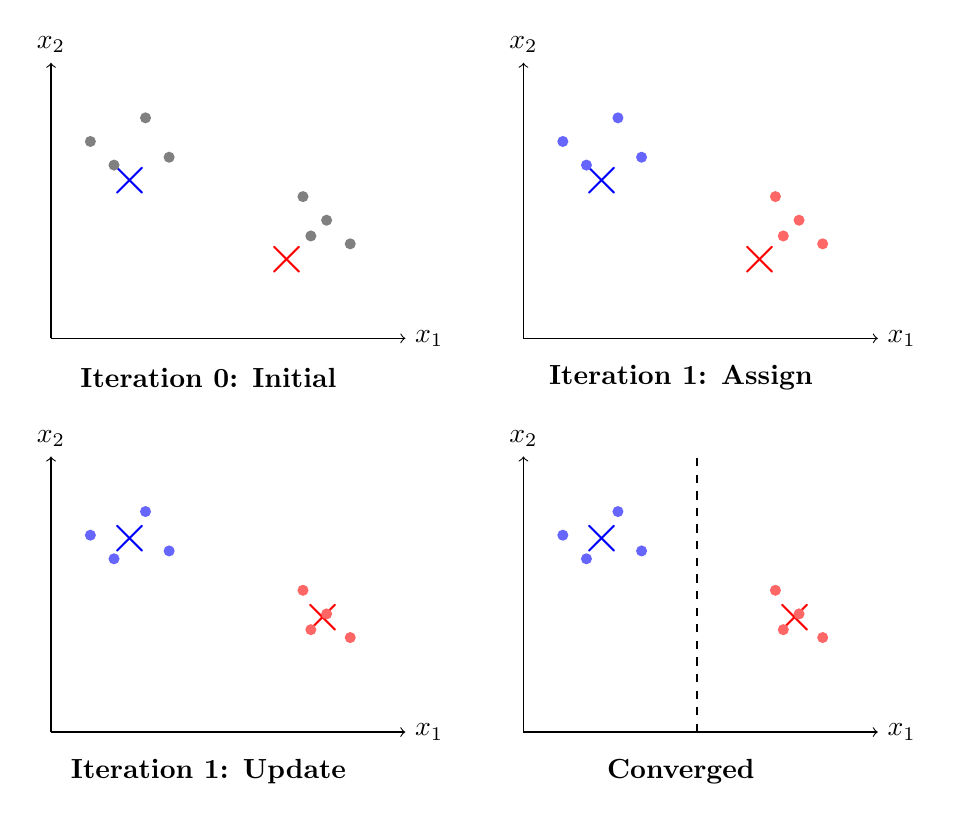
\begin{tikzpicture}[scale=1.0]
    % Initial state
    \begin{scope}
        \node at (2, -0.5) {\textbf{Iteration 0: Initial}};
        
        % Random centroids
        \node[text=blue,font=\bfseries,scale=2] at (1,2) {$\times$};
        \node[text=red,font=\bfseries,scale=2] at (3,1) {$\times$};
        
        % Data points (not yet colored)
        \foreach \x/\y in {0.5/2.5, 0.8/2.2, 1.2/2.8, 1.5/2.3, 
                           3.5/1.5, 3.2/1.8, 3.8/1.2, 3.3/1.3} {
            \fill[gray] (\x,\y) circle (2pt);
        }
        
        \draw[->] (0,0) -- (4.5,0) node[right] {$x_1$};
        \draw[->] (0,0) -- (0,3.5) node[above] {$x_2$};
    \end{scope}
    
    % After assignment
    \begin{scope}[xshift=6cm]
        \node at (2, -0.5) {\textbf{Iteration 1: Assign}};
        
        % Centroids (same position)
        \node[text=blue,font=\bfseries,scale=2] at (1,2) {$\times$};
        \node[text=red,font=\bfseries,scale=2] at (3,1) {$\times$};
        
        % Data points colored by assignment
        \foreach \x/\y in {0.5/2.5, 0.8/2.2, 1.2/2.8, 1.5/2.3} {
            \fill[blue!60] (\x,\y) circle (2pt);
        }
        \foreach \x/\y in {3.5/1.5, 3.2/1.8, 3.8/1.2, 3.3/1.3} {
            \fill[red!60] (\x,\y) circle (2pt);
        }
        
        \draw[->] (0,0) -- (4.5,0) node[right] {$x_1$};
        \draw[->] (0,0) -- (0,3.5) node[above] {$x_2$};
    \end{scope}
    
    % After update
    \begin{scope}[yshift=-5cm]
        \node at (2, -0.5) {\textbf{Iteration 1: Update}};
        
        % Updated centroids
        \node[text=blue,font=\bfseries,scale=2] at (1,2.45) {$\times$};
        \node[text=red,font=\bfseries,scale=2] at (3.45,1.45) {$\times$};
        
        % Data points
        \foreach \x/\y in {0.5/2.5, 0.8/2.2, 1.2/2.8, 1.5/2.3} {
            \fill[blue!60] (\x,\y) circle (2pt);
        }
        \foreach \x/\y in {3.5/1.5, 3.2/1.8, 3.8/1.2, 3.3/1.3} {
            \fill[red!60] (\x,\y) circle (2pt);
        }
        
        \draw[->] (0,0) -- (4.5,0) node[right] {$x_1$};
        \draw[->] (0,0) -- (0,3.5) node[above] {$x_2$};
    \end{scope}
    
    % Converged state
    \begin{scope}[xshift=6cm, yshift=-5cm]
        \node at (2, -0.5) {\textbf{Converged}};
        
        % Final centroids
        \node[text=blue,font=\bfseries,scale=2] at (1,2.45) {$\times$};
        \node[text=red,font=\bfseries,scale=2] at (3.45,1.45) {$\times$};
        
        % Voronoi boundaries (conceptual)
        \draw[dashed, thick] (2.2, 0) -- (2.2, 3.5);
        
    % cleaned trailing markdown fences
        \foreach \x/\y in {0.5/2.5, 0.8/2.2, 1.2/2.8, 1.5/2.3} {
            \fill[blue!60] (\x,\y) circle (2pt);
        }
        \foreach \x/\y in {3.5/1.5, 3.2/1.8, 3.8/1.2, 3.3/1.3} {
            \fill[red!60] (\x,\y) circle (2pt);
        }
        
        \draw[->] (0,0) -- (4.5,0) node[right] {$x_1$};
        \draw[->] (0,0) -- (0,3.5) node[above] {$x_2$};
    \end{scope}
\end{tikzpicture}
\end{center}

The four panels show k-means progression: random initialization, assignment to nearest centroid, centroid update, and final convergence with Voronoi partition.
\end{visualbox}

\subsection{Code Implementation}

\begin{codebox}
\textbf{K-Means Clustering in Python (Scikit-Learn):}

\begin{lstlisting}
import numpy as np
import matplotlib.pyplot as plt
from sklearn.cluster import KMeans
from sklearn.datasets import make_blobs

# Generate synthetic data with 3 natural clusters
X, y_true = make_blobs(n_samples=300, centers=3, 
                       cluster_std=0.6, random_state=42)

# Apply K-Means
kmeans = KMeans(n_clusters=3, random_state=42, n_init=10)
kmeans.fit(X)

# Extract results
labels = kmeans.labels_
centroids = kmeans.cluster_centers_
inertia = kmeans.inertia_

print(f"Final inertia (within-cluster sum of squares): {inertia:.2f}")
print(f"Centroid positions:\n{centroids}")

# Visualization
plt.figure(figsize=(10, 5))

# Subplot 1: True labels
plt.subplot(1, 2, 1)
plt.scatter(X[:, 0], X[:, 1], c=y_true, cmap='viridis', 
            alpha=0.6, edgecolors='k')
plt.title("True Clusters (Ground Truth)")
plt.xlabel("Feature 1")
plt.ylabel("Feature 2")

# Subplot 2: K-Means prediction
plt.subplot(1, 2, 2)
plt.scatter(X[:, 0], X[:, 1], c=labels, cmap='viridis', 
            alpha=0.6, edgecolors='k')
plt.scatter(centroids[:, 0], centroids[:, 1], c='red', 
            marker='X', s=200, edgecolors='black', 
            label='Centroids')
plt.title("K-Means Clustering Result")
plt.xlabel("Feature 1")
plt.ylabel("Feature 2")
plt.legend()

plt.tight_layout()
plt.show()
\end{lstlisting}

\textbf{Philosophical Meditation:} Run this code multiple times with different \texttt{random\_state} values. Observe how initialization affects final clustering---epistemic uncertainty made visible.
\end{codebox}

\begin{codebox}
\textbf{K-Means on High-Dimensional Data (with PCA):}

\begin{lstlisting}
from sklearn.decomposition import PCA
from sklearn.preprocessing import StandardScaler

# Generate high-dimensional data (9 features)
X_high = np.random.randn(500, 9)
# Add structure: first 3 features determine cluster
X_high[:250, :3] += 3  # Cluster 1
X_high[250:, :3] -= 3  # Cluster 2

# Standardize features
scaler = StandardScaler()
X_scaled = scaler.fit_transform(X_high)

# Apply K-Means in full space
kmeans_full = KMeans(n_clusters=2, random_state=42)
labels_full = kmeans_full.fit_predict(X_scaled)

# Reduce to 2D for visualization
pca = PCA(n_components=2)
X_2d = pca.fit_transform(X_scaled)

print(f"Explained variance ratio: {pca.explained_variance_ratio_}")
print(f"Total variance explained: {pca.explained_variance_ratio_.sum():.2%}")

# Visualize
plt.figure(figsize=(8, 6))
plt.scatter(X_2d[:, 0], X_2d[:, 1], c=labels_full, 
            cmap='coolwarm', alpha=0.7, edgecolors='k')
plt.title("K-Means Clustering (9D data, PCA projection to 2D)")
plt.xlabel(f"PC1 ({pca.explained_variance_ratio_[0]:.1%} variance)")
plt.ylabel(f"PC2 ({pca.explained_variance_ratio_[1]:.1%} variance)")
plt.colorbar(label='Cluster')
plt.show()
\end{lstlisting}

\textbf{Key Insight:} PCA preserves the clustering structure if the discriminative features have high variance. The explained variance ratio tells us how much information is retained in the 2D projection.
\end{codebox}

\section{Hierarchical Clustering: Taxonomy of Similarity}

\subsection{Agglomerative Clustering}

Unlike k-means, hierarchical clustering does not require specifying $k$ in advance. Instead, it builds a \textit{dendrogram}---a tree structure revealing nested relationships.

\begin{seanbox}{4.2}
\textbf{Agglomerative Hierarchical Clustering:}

\textbf{Algorithm (Bottom-Up):}

\begin{enumerate}
    \item \textbf{Initialize:} Start with each point as its own cluster
    \begin{equation}
        \mathcal{C}_0 = \{\{x^{(1)}\}, \{x^{(2)}\}, \ldots, \{x^{(m)}\}\}
    \end{equation}
    
    \item \textbf{Repeat until one cluster remains:}
    \begin{enumerate}
        \item Find the two closest clusters $C_i, C_j$ according to linkage criterion
        \item Merge them: $C_{\text{new}} = C_i \cup C_j$
        \item Update cluster set: $\mathcal{C} \leftarrow (\mathcal{C} \setminus \{C_i, C_j\}) \cup \{C_{\text{new}}\}$
    \end{enumerate}
\end{enumerate}

\textbf{Linkage Criteria (Distance between clusters):}

\begin{itemize}
    \item \textbf{Single Linkage:} Minimum distance between any two points
    \begin{equation}
        d(C_i, C_j) = \min_{\vect{x} \in C_i, \vect{y} \in C_j} \|\vect{x} - \vect{y}\|
    \end{equation}
    
    \item \textbf{Complete Linkage:} Maximum distance (diameter)
    \begin{equation}
        d(C_i, C_j) = \max_{\vect{x} \in C_i, \vect{y} \in C_j} \|\vect{x} - \vect{y}\|
    \end{equation}
    
    \item \textbf{Average Linkage:} Mean distance
    \begin{equation}
        d(C_i, C_j) = \frac{1}{|C_i||C_j|} \sum_{\vect{x} \in C_i} \sum_{\vect{y} \in C_j} \|\vect{x} - \vect{y}\|
    \end{equation}
    
    \item \textbf{Ward's Method:} Minimizes within-cluster variance increase
    \begin{equation}
        d(C_i, C_j) = \frac{|C_i||C_j|}{|C_i| + |C_j|} \|\mu_i - \mu_j\|^2
    \end{equation}
\end{itemize}
\end{seanbox}

\begin{philobox}
\textbf{Hierarchical Clustering as Ontological Taxonomy}

Linnaeus classified organisms into nested categories: species, genus, family, order, class, phylum, kingdom. Hierarchical clustering formalizes this intuition:

\begin{itemize}
    \item \textbf{Leaves (individuals)}: Data points are the most specific level
    \item \textbf{Internal nodes (categories)}: Clusters represent increasing levels of abstraction
    \item \textbf{Root (universal)}: The final merged cluster encompasses all data
\end{itemize}

The dendrogram is an \textit{ontological map}---a visualization of how particulars relate to universals through nested containment. The height at which clusters merge indicates their dissimilarity---a geometric encoding of conceptual distance.

This mirrors Porphyry's \textit{Tree of Categories} and medieval scholastic debates about genus and species. The notation $C_{\text{new}} = C_i \cup C_j$ captures \textit{categorical subsumption}.
\end{philobox}

\subsection{Dendrogram Visualization}

\begin{visualbox}
\textbf{Dendrogram Structure:}

\begin{center}
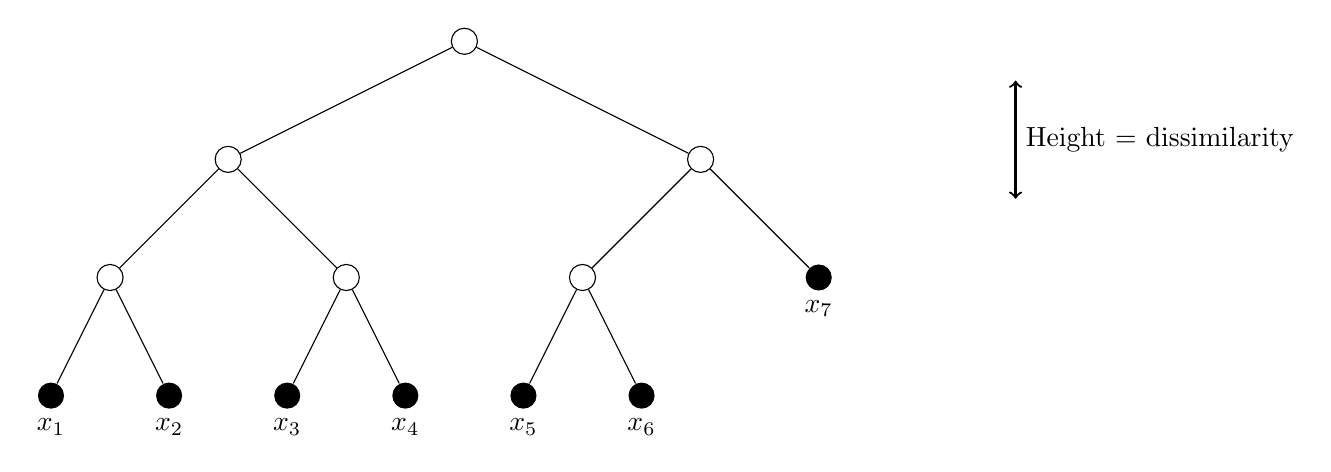
\begin{tikzpicture}[
    level distance=1.5cm,
    level 1/.style={sibling distance=6cm},
    level 2/.style={sibling distance=3cm},
    level 3/.style={sibling distance=1.5cm}
]
    \node[circle, draw] (root) {}
        child {
            node[circle, draw] {}
            child {
                node[circle, draw] {}
                child {node[circle, fill, label=below:$x_1$] {}}
                child {node[circle, fill, label=below:$x_2$] {}}
            }
            child {
                node[circle, draw] {}
                child {node[circle, fill, label=below:$x_3$] {}}
                child {node[circle, fill, label=below:$x_4$] {}}
            }
        }
        child {
            node[circle, draw] {}
            child {
                node[circle, draw] {}
                child {node[circle, fill, label=below:$x_5$] {}}
                child {node[circle, fill, label=below:$x_6$] {}}
            }
            child {node[circle, fill, label=below:$x_7$] {}}
        };
    
    % Add height annotations
    \draw[<->, thick] (7, -0.5) -- (7, -2.0) node[midway, right] {Height = dissimilarity};
\end{tikzpicture}
\end{center}

Vertical axis represents dissimilarity at merge. Cutting horizontally at any height produces a flat clustering.
\end{visualbox}

\subsection{Code Implementation}

\begin{codebox}
\textbf{Hierarchical Clustering with Dendrogram:}

\begin{lstlisting}
import numpy as np
import matplotlib.pyplot as plt
from scipy.cluster.hierarchy import dendrogram, linkage
from sklearn.cluster import AgglomerativeClustering

# Generate sample data
np.random.seed(42)
X = np.random.randn(50, 2)
X[:25, :] += 3  # Create structure

# Compute linkage matrix (for dendrogram)
Z = linkage(X, method='ward')

# Plot dendrogram
plt.figure(figsize=(12, 5))

plt.subplot(1, 2, 1)
dendrogram(Z)
plt.title("Hierarchical Clustering Dendrogram")
plt.xlabel("Sample Index")
plt.ylabel("Distance (Ward)")

# Apply hierarchical clustering with cut at k=2
hierarchical = AgglomerativeClustering(n_clusters=2, linkage='ward')
labels = hierarchical.fit_predict(X)

# Plot clusters
plt.subplot(1, 2, 2)
plt.scatter(X[:, 0], X[:, 1], c=labels, cmap='viridis', 
            alpha=0.7, edgecolors='k')
plt.title("Hierarchical Clustering Result (k=2)")
plt.xlabel("Feature 1")
plt.ylabel("Feature 2")

plt.tight_layout()
plt.show()
\end{lstlisting}

\textbf{Reflection:} The dendrogram lets you choose the number of clusters \textit{post hoc} by cutting at different heights---epistemic flexibility.
\end{codebox}

\section{DBSCAN: Density-Based Clustering}

\subsection{Beyond Spherical Clusters}

K-means assumes spherical, equally-sized clusters. DBSCAN (Density-Based Spatial Clustering of Applications with Noise) handles arbitrary shapes and automatically detects outliers.

\begin{seanbox}{4.3}
\textbf{DBSCAN Algorithm:}

\textbf{Parameters:}
\begin{itemize}
    \item $\epsilon$: Neighborhood radius
    \item $\text{minPts}$: Minimum points to form dense region
\end{itemize}

\textbf{Point Classifications:}

\begin{itemize}
    \item \textbf{Core point}: Has at least minPts neighbors within $\epsilon$
    \begin{equation}
        |\{\vect{x}^{(j)} : \|\vect{x}^{(i)} - \vect{x}^{(j)}\| \leq \epsilon\}| \geq \text{minPts}
    \end{equation}
    
    \item \textbf{Border point}: Within $\epsilon$ of a core point, but not itself core
    
    \item \textbf{Noise point}: Neither core nor border
\end{itemize}

\textbf{Algorithm:}

\begin{enumerate}
    \item Label all points as core, border, or noise
    \item Create edge between core points within $\epsilon$ of each other
    \item Each connected component of core points forms a cluster
    \item Assign border points to nearby clusters
    \item Mark noise points as outliers (cluster label = -1)
\end{enumerate}
\end{seanbox}

\begin{philobox}
\textbf{DBSCAN and Topological Intuition}

DBSCAN embodies \textit{topological thinking}---clustering based on connectivity rather than centroids:

\begin{itemize}
    \item \textbf{Dense regions = manifolds}: Clusters are locally dense manifolds in feature space
    \item \textbf{Low-density regions = boundaries}: Natural separations between clusters
    \item \textbf{Noise = singularities}: Outliers that don't belong to any manifold
\end{itemize}

This approach resonates with Heidegger's \textit{Being-in-the-world}: entities are defined not by essential properties (centroids) but by their \textit{nearness} to others---their position in a relational network.

The notation $\epsilon$-neighborhood captures \textit{locality}: what matters is ``Who are my neighbors?'' not ``What is my distance to an ideal?''
\end{philobox}

\subsection{Code Implementation}

\begin{codebox}
\textbf{DBSCAN on Non-Spherical Clusters:}

\begin{lstlisting}
from sklearn.cluster import DBSCAN
from sklearn.datasets import make_moons

# Generate moon-shaped data (non-convex clusters)
X, y_true = make_moons(n_samples=300, noise=0.05, random_state=42)

# Apply DBSCAN
dbscan = DBSCAN(eps=0.2, min_samples=5)
labels = dbscan.fit_predict(X)

# Count clusters and noise points
n_clusters = len(set(labels)) - (1 if -1 in labels else 0)
n_noise = list(labels).count(-1)

print(f"Estimated number of clusters: {n_clusters}")
print(f"Estimated number of noise points: {n_noise}")

# Visualization
plt.figure(figsize=(12, 5))

plt.subplot(1, 2, 1)
plt.scatter(X[:, 0], X[:, 1], c=y_true, cmap='viridis', 
            alpha=0.7, edgecolors='k')
plt.title("True Labels (Moon Dataset)")

plt.subplot(1, 2, 2)
plt.scatter(X[:, 0], X[:, 1], c=labels, cmap='plasma', 
            alpha=0.7, edgecolors='k')
plt.title(f"DBSCAN Result (eps={dbscan.eps}, minPts={dbscan.min_samples})")

plt.tight_layout()
plt.show()
\end{lstlisting}

\textbf{Key Observation:} DBSCAN successfully separates the two moons, while k-means would fail. This demonstrates the importance of choosing algorithms aligned with data geometry.
\end{codebox}

\section{Gaussian Mixture Models: Probabilistic Clustering}

\subsection{Soft Clustering via Probability}

GMMs extend k-means by:
\begin{enumerate}
    \item Allowing \textit{soft assignments} (probabilities rather than hard labels)
    \item Modeling each cluster as a Gaussian distribution
    \item Learning cluster covariances (not just spherical)
\end{enumerate}

\begin{seanbox}{4.4}
\textbf{Gaussian Mixture Model:}

\textbf{Model:} Data generated from mixture of $k$ Gaussians

\begin{equation}
    p(\vect{x}) = \sum_{j=1}^k \pi_j \mathcal{N}(\vect{x} \mid \mu_j, \Sigma_j)
\end{equation}

where:
\begin{itemize}
    \item $\pi_j$: Mixing coefficient (prior probability of cluster $j$), $\sum_j \pi_j = 1$
    \item $\mu_j$: Mean of Gaussian $j$
    \item $\Sigma_j$: Covariance matrix of Gaussian $j$
    \item $\mathcal{N}(\vect{x} \mid \mu, \Sigma)$: Multivariate Gaussian density
\end{itemize}

\textbf{Posterior Probability (Responsibility):}

\begin{equation}
    \gamma_{ij} = P(z^{(i)} = j \mid \vect{x}^{(i)}) = \frac{\pi_j \mathcal{N}(\vect{x}^{(i)} \mid \mu_j, \Sigma_j)}{\sum_{k=1}^K \pi_k \mathcal{N}(\vect{x}^{(i)} \mid \mu_k, \Sigma_k)}
\end{equation}

This is the \textit{soft assignment}: probability that point $i$ belongs to cluster $j$.

\textbf{Expectation-Maximization (EM) Algorithm:}

\textbf{E-step:} Compute responsibilities $\gamma_{ij}$ given current parameters

\textbf{M-step:} Update parameters given responsibilities

\begin{align}
    \pi_j &= \frac{1}{m} \sum_{i=1}^m \gamma_{ij} \\
    \mu_j &= \frac{\sum_{i=1}^m \gamma_{ij} \vect{x}^{(i)}}{\sum_{i=1}^m \gamma_{ij}} \\
    \Sigma_j &= \frac{\sum_{i=1}^m \gamma_{ij} (\vect{x}^{(i)} - \mu_j)(\vect{x}^{(i)} - \mu_j)^\top}{\sum_{i=1}^m \gamma_{ij}}
\end{align}

Iterate until convergence.
\end{seanbox}

\begin{philobox}
\textbf{GMM as Fuzzy Logic}

Unlike k-means (``Point $i$ IS in cluster $j$''), GMM assigns a probability to membership rather than a hard label.

% Promotional Markdown/emoji block removed. Kept the scholarly text; if you want a LaTeX-native summary box
% we can add it instead. The removed content contained backticks, Markdown headings and emoji (✅)
% which break LaTeX compilation. See git history to recover if needed.

Lotfi Zadeh's fuzzy set theory (1965) challenged classical bivalent logic: membership is not binary but graded. GMM operationalizes this:

\begin{equation}
    \text{Membership}(x^{(i)} \in C_j) = \gamma_{ij} \in [0, 1]
\end{equation}

This philosophical shift acknowledges \textit{epistemic uncertainty}: we cannot perfectly classify every point, so we quantify our uncertainty probabilistically.

The notation $\mathcal{N}(\vect{x} \mid \mu, \Sigma)$ emphasizes that clusters are not point masses (centroids) but \textit{probability distributions}---extended regions with varying density.
\end{philobox}

\subsection{Code Implementation}

\begin{codebox}
\textbf{Gaussian Mixture Model with Soft Assignments:}

\begin{lstlisting}
from sklearn.mixture import GaussianMixture

# Generate data with different cluster shapes
np.random.seed(42)
X1 = np.random.randn(150, 2) * 0.5 + [0, 0]
X2 = np.random.randn(150, 2) * [[2, 0.5], [0.5, 1]] + [4, 4]
X = np.vstack([X1, X2])

# Fit GMM
gmm = GaussianMixture(n_components=2, covariance_type='full', random_state=42)
gmm.fit(X)

# Hard assignments (most probable cluster)
labels_hard = gmm.predict(X)

# Soft assignments (probabilities)
probs = gmm.predict_proba(X)

print(f"Mixing coefficients (pi): {gmm.weights_}")
print(f"Means:\n{gmm.means_}")
print(f"Covariances:\n{gmm.covariances_}")

# Visualization
fig, axes = plt.subplots(1, 3, figsize=(15, 5))

# Hard clustering
axes[0].scatter(X[:, 0], X[:, 1], c=labels_hard, cmap='viridis', 
                alpha=0.6, edgecolors='k')
axes[0].scatter(gmm.means_[:, 0], gmm.means_[:, 1], c='red', 
                marker='X', s=200, edgecolors='black')
axes[0].set_title("GMM: Hard Clustering")

# Soft clustering (color by probability of cluster 0)
axes[1].scatter(X[:, 0], X[:, 1], c=probs[:, 0], cmap='coolwarm', 
                alpha=0.7, edgecolors='k')
axes[1].set_title("GMM: Probability of Cluster 0")
axes[1].colorbar = plt.colorbar(ax=axes[1], label='P(cluster 0)')

# Uncertainty (entropy of assignment)
entropy = -np.sum(probs * np.log(probs + 1e-10), axis=1)
axes[2].scatter(X[:, 0], X[:, 1], c=entropy, cmap='plasma', 
                alpha=0.7, edgecolors='k')
axes[2].set_title("GMM: Assignment Uncertainty (Entropy)")

plt.tight_layout()
plt.show()
\end{lstlisting}

\textbf{Philosophical Insight:} The entropy plot reveals points near cluster boundaries---regions of maximum epistemic uncertainty.
\end{codebox}

\section{Choosing the Number of Clusters}

\subsection{The Elbow Method}

\begin{definition}[Within-Cluster Sum of Squares (WCSS)]
For k-means clustering:

\begin{equation}
    \text{WCSS}(k) = \sum_{j=1}^k \sum_{i \in C_j} \|\vect{x}^{(i)} - \mu_j\|^2
\end{equation}

As $k$ increases, WCSS decreases (more clusters = tighter fit). The \textit{elbow point} is where returns diminish.
\end{definition}

\begin{visualbox}
\textbf{Elbow Method Visualization:}

\begin{center}
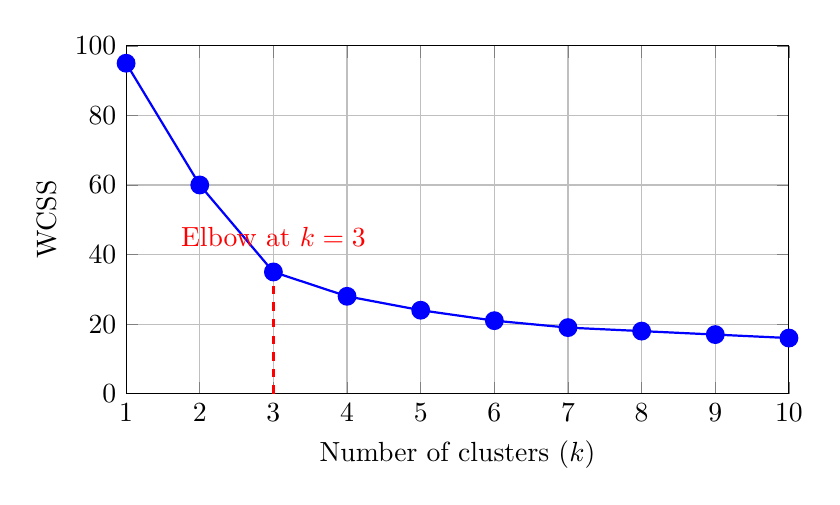
\begin{tikzpicture}
    \begin{axis}[
        width=10cm,
        height=6cm,
        xlabel={Number of clusters ($k$)},
        ylabel={WCSS},
        xmin=1, xmax=10,
        ymin=0, ymax=100,
        xtick={1,2,3,4,5,6,7,8,9,10},
        grid=major
    ]
    
    % Elbow curve (decreasing exponentially)
    \addplot[blue, thick, mark=*, mark options={scale=1.5}] coordinates {
        (1, 95)
        (2, 60)
        (3, 35)  % Elbow here
        (4, 28)
        (5, 24)
        (6, 21)
        (7, 19)
        (8, 18)
        (9, 17)
        (10, 16)
    };
    
    % Highlight elbow
    \draw[red, thick, dashed] (axis cs:3,0) -- (axis cs:3,35);
    \node[red] at (axis cs:3, 45) {Elbow at $k=3$};
    
    \end{axis}
\end{tikzpicture}
\end{center}

The elbow at $k=3$ suggests the data has 3 natural clusters. Beyond this, adding clusters yields diminishing improvement.
\end{visualbox}

\subsection{Silhouette Score}

\begin{definition}[Silhouette Coefficient]
For point $i$ in cluster $C_j$:

\begin{align}
    a_i &= \frac{1}{|C_j| - 1} \sum_{k \in C_j, k \neq i} \|\vect{x}^{(i)} - \vect{x}^{(k)}\| \quad \text{(intra-cluster distance)} \\
    b_i &= \min_{j' \neq j} \frac{1}{|C_{j'}|} \sum_{k \in C_{j'}} \|\vect{x}^{(i)} - \vect{x}^{(k)}\| \quad \text{(nearest other cluster)} \\
    s_i &= \frac{b_i - a_i}{\max(a_i, b_i)}
\end{align}

Average silhouette score: $\bar{s} = \frac{1}{m} \sum_{i=1}^m s_i$

\textbf{Interpretation:}
\begin{itemize}
    \item $s_i \approx 1$: Well-clustered (far from other clusters)
    \item $s_i \approx 0$: On cluster boundary
    \item $s_i < 0$: Likely misclassified
\end{itemize}
\end{definition}

\begin{codebox}
\textbf{Elbow Method and Silhouette Analysis:}

\begin{lstlisting}
from sklearn.metrics import silhouette_score

# Range of k to try
k_range = range(2, 11)
wcss_values = []
silhouette_scores = []

for k in k_range:
    kmeans = KMeans(n_clusters=k, random_state=42, n_init=10)
    labels = kmeans.fit_predict(X)
    
    wcss_values.append(kmeans.inertia_)
    silhouette_scores.append(silhouette_score(X, labels))

# Plot results
fig, axes = plt.subplots(1, 2, figsize=(12, 5))

# Elbow plot
axes[0].plot(k_range, wcss_values, 'bo-', linewidth=2, markersize=8)
axes[0].set_xlabel('Number of clusters (k)')
axes[0].set_ylabel('WCSS')
axes[0].set_title('Elbow Method')
axes[0].grid(True)

# Silhouette plot
axes[1].plot(k_range, silhouette_scores, 'ro-', linewidth=2, markersize=8)
axes[1].set_xlabel('Number of clusters (k)')
axes[1].set_ylabel('Average Silhouette Score')
axes[1].set_title('Silhouette Analysis')
axes[1].grid(True)

plt.tight_layout()
plt.show()

# Find optimal k
optimal_k = k_range[np.argmax(silhouette_scores)]
print(f"Optimal k by silhouette score: {optimal_k}")
\end{lstlisting}
\end{codebox}

\section{Practical Considerations and Challenges}

\subsection{The Curse of Dimensionality}

\begin{remark}[High-Dimensional Clustering]
In high dimensions ($d \gg 10$), distance metrics become less discriminative:

\begin{equation}
    \lim_{d \to \infty} \frac{\text{dist}_{\max} - \text{dist}_{\min}}{\text{dist}_{\min}} \to 0
\end{equation}

All points appear equidistant! This is the \textbf{curse of dimensionality}.

\textbf{Solutions:}
\begin{itemize}
    \item \textbf{Dimensionality reduction:} PCA, t-SNE, UMAP before clustering
    \item \textbf{Feature selection:} Identify discriminative features
    \item \textbf{Subspace clustering:} Find clusters in different subspaces
\end{itemize}
\end{remark}

\subsection{Comparing Clustering Algorithms}

\begin{table}[h]
\centering
\caption{Comparison of Clustering Algorithms}
\begin{tabular}{|l|c|c|c|c|}
\hline
\textbf{Algorithm} & \textbf{Cluster Shape} & \textbf{Needs $k$?} & \textbf{Handles Noise?} & \textbf{Complexity} \\ \hline
K-Means & Spherical & Yes & No & $O(mkd)$ \\ \hline
Hierarchical & Any & No & No & $O(m^2 \log m)$ \\ \hline
DBSCAN & Arbitrary & No & Yes & $O(m \log m)$ \\ \hline
GMM & Ellipsoidal & Yes & Soft & $O(mkd^2)$ \\ \hline
\end{tabular}
\end{table}

\subsection{Irreducible Error in Clustering}

\begin{philosophical}
Even with perfect algorithms, clustering faces \textbf{irreducible error}:

\begin{enumerate}
    \item \textbf{Ontological ambiguity:} Data may not have ``true'' clusters. Natural kinds are not always discrete.
    
    \item \textbf{Information loss:} Dimensionality reduction discards information. PCA preserves variance, not necessarily cluster structure.
    
    \item \textbf{Epistemic limits:} Missing features prevent perfect separation. We cluster based on observed features, but latent factors may be unobserved.
\end{enumerate}

This echoes Hume's \textit{problem of induction}: we generalize from finite samples to infinite populations, always with residual uncertainty. Clustering reveals structure \textit{relative to our measurement apparatus and chosen similarity metric}---not absolute truth.
\end{philosophical}

\section{Advanced Topics}

\subsection{Spectral Clustering}

\begin{definition}[Spectral Clustering]
Uses eigenvectors of similarity matrix (graph Laplacian) to embed data, then applies k-means in embedding space.

\textbf{Key Idea:} Transform data so that clusters become linearly separable in spectral embedding.
\end{definition}

\begin{codebox}
\begin{lstlisting}
from sklearn.cluster import SpectralClustering

# Apply spectral clustering
spectral = SpectralClustering(n_clusters=2, affinity='nearest_neighbors', 
                               n_neighbors=10, random_state=42)
labels_spectral = spectral.fit_predict(X)

plt.scatter(X[:, 0], X[:, 1], c=labels_spectral, cmap='viridis', 
            alpha=0.7, edgecolors='k')
plt.title("Spectral Clustering")
plt.show()
\end{lstlisting}
\end{codebox}

\subsection{Consensus Clustering}

\begin{definition}[Consensus Clustering]
Run clustering algorithm multiple times with different initializations or subsamples, then aggregate results to find robust clusters.

\textbf{Philosophy:} If a cluster appears consistently across many trials, it is more likely to reflect genuine structure (not algorithmic artifact).
\end{definition}

\section{Reflective Exercises}

\begin{exercise}[K-Means Sensitivity]
Generate a dataset with 3 clusters. Run k-means 100 times with random initializations. How often does it find the global optimum? What does this reveal about the reliability of clustering?
\end{exercise}

\begin{exercise}[Linkage Criterion Comparison]
Apply hierarchical clustering with single, complete, average, and Ward linkage to the same dataset. Compare dendrograms. Which criterion produces the most interpretable result? Why might different criteria favor different structures?
\end{exercise}

\begin{exercise}[DBSCAN Parameter Tuning]
For a given dataset, systematically vary $\epsilon$ and minPts. Plot the number of clusters found vs. parameter values. How sensitive is DBSCAN to parameter choice? What philosophical implications does this sensitivity have?
\end{exercise}

\begin{exercise}[Philosophical: Natural Kinds]
Do clusters discovered by algorithms correspond to ``natural kinds'' (Plato's Forms, Aristotle's species)? Or are they human-imposed categories? Discuss with reference to a real-world application (e.g., gene expression clusters, customer segments).
\end{exercise}

\begin{exercise}[GMM vs. K-Means]
On the same dataset, apply both GMM and k-means. Identify points where they disagree. Inspect these points manually---are they genuinely ambiguous? Does soft clustering (GMM) provide epistemically honest uncertainty quantification?
\end{exercise}

\begin{exercise}[High-Dimensional Clustering]
Generate a 100-dimensional dataset with 3 clusters (signal only in first 5 dimensions, rest noise). Apply:
\begin{enumerate}
    \item K-means on raw data
    \item PCA reduction to 5D, then k-means
    \item Feature selection (pick 5 most variant features), then k-means
\end{enumerate}
Compare results. What does this teach about the curse of dimensionality?
\end{exercise}

\begin{exercise}[Coding: Implement Lloyd's Algorithm]
Write k-means from scratch (no sklearn). Implement:
\begin{itemize}
    \item Random initialization
    \item Assignment step
    \item Update step
    \item Convergence check
\end{itemize}
Visualize centroid positions at each iteration (animate if possible). This exercise builds intuition for the iterative refinement process.
\end{exercise}

\section{Connections to Other Parts}

\subsection{To Part I (Linear Algebra)}
\begin{itemize}
    \item K-means centroids are computed via matrix operations (averaging = multiplication by $\frac{1}{m}\vect{1}^\top$)
    \item Covariance matrices in GMM are symmetric positive semi-definite
    \item Spectral clustering uses eigendecomposition of graph Laplacian
\end{itemize}

\subsection{To Part II (Statistics)}
\begin{itemize}
    \item GMM is maximum likelihood estimation of mixture model parameters
    \item Silhouette score is a statistical measure of cluster quality
    \item EM algorithm for GMM alternates between E-step (expectation) and M-step (maximization)
\end{itemize}

\subsection{To Part III (Computer Vision)}
\begin{itemize}
    \item Image segmentation is clustering in pixel space (color + position)
    \item K-means used for color quantization (reducing palette)
    \item Attention mechanisms create soft clusters of related tokens
\end{itemize}

\subsection{To Part V (Reinforcement Learning)}
\begin{itemize}
    \item State abstraction in RL uses clustering to group similar states
    \item Behavioral cloning clusters expert demonstrations to identify distinct strategies
    \item Hierarchical RL uses clustering to discover sub-goals
\end{itemize}

\subsection{To Part VI (Vector Calculus)}
\begin{itemize}
    \item Gradient descent used in k-means optimization (implicitly)
    \item Laplacian operator in spectral clustering relates to diffusion on graphs
    \item Gaussian distributions in GMM are exponentials of quadratic forms (related to harmonic oscillators)
\end{itemize}

\section{Conclusion: Clustering as Epistemic Tool}

Clustering is more than an algorithm---it is a \textbf{way of seeing}. By partitioning data into groups, we impose structure on chaos, reveal patterns in noise, and ascend from the particular to the universal.

\textbf{Key Insights:}

\begin{enumerate}
    \item \textbf{Philosophical:} Clustering formalizes the ancient quest to discover natural kinds---categories that ``carve nature at its joints.''
    
    \item \textbf{Epistemological:} Data are the seeds of knowledge; clustering is the analytical process that cultivates these seeds into insight.
    
    \item \textbf{Mathematical:} Different algorithms embody different assumptions about cluster geometry (spherical, hierarchical, density-based, probabilistic).
    
    \item \textbf{Practical:} No single algorithm is universally best. The choice depends on data structure, domain knowledge, and interpretability requirements.
    
    \item \textbf{Limitations:} Clustering faces irreducible error due to epistemic limits, ontological ambiguity, and the curse of dimensionality.
\end{enumerate}

\begin{center}
\itshape
``In clustering, we do not discover truth—we create interpretations. \\
The map is not the territory, but a good map reveals the territory's structure. \\
Our algorithms are lenses through which data's latent order becomes visible.''
\end{center}

\vspace{1cm}

As you apply these techniques, remember: clustering is an \textit{art} informed by science. The notation guides computation, but \textit{interpretation} requires domain expertise, philosophical reflection, and epistemic humility. The clusters you discover are hypotheses about reality---testable, revisable, and always incomplete.

\clearpage
